
%
% Beispieldokument für TU beamer theme
%
% v1.0: 12.10.2014
% 
\documentclass[xcolor={dvipsnames}]{beamer}
\usetheme{TU}

\usepackage{booktabs}
\usepackage{tabularx}
% Macro to make entire row bold from https://tex.stackexchange.com/questions/309833/format-whole-row-of-table-as-bold
\newcommand\setrow[1]{\gdef\rowmac{#1}#1\ignorespaces}
\newcommand\clearrow{\global\let\rowmac\relax}
\clearrow

\title{SparseIDS: Learning Packet Sampling with Reinforcement Learning}

\author[M. Bachl et al.]{%
	\underline{Maximilian Bachl}\email{maximilian.bachl@tuwien.ac.at} \and Fares Meghdouri \and Tanja Zseby \and Joachim Fabini
}

\institute{%
	Technische Universität Wien, Vienna, Austria
}

%\session{XXXX \#}

%Kann angepasst werden, wie es beliebt. Entweder das Datum der Präsentation oder das Datum der aktuellen Präsentations-Version.
%\date[\the\day.\the\month.\the\year]{\today}
\date[July 1, 2020]{July 1, 2020}

\begin{document}

\maketitle

\section{Introduction}

\begin{frame}{Recurrent Neural Networks (RNNs)}
\begin{itemize}
\item RNNs are neural networks for \textbf{sequences}
\item Good performance for network traffic \footnote{\textit{Explainability and Adversarial Robustness for RNNs}, Hartl, Bachl, Fabini, Zseby, 2020} with \textbf{supervised} training
\item Can detect intrusion \textbf{before} an attack is over
\end{itemize}
\end{frame}

\begin{frame}{Sampling for RNNs}
\begin{itemize}
\item Processing every packet by a neural network is \textbf{resource-intensive}
\item Often, attack is apparent after the first packets of a flow $\rightarrow$ not \textbf{necessary} to continue inspecting packets
\item Some packets might contain \textbf{no information} that is useful for classification
\end{itemize}
\pause
\begin{block}{Goal:}
Only process packets if they are useful for the classifier! 
\end{block}
\end{frame}

\section{Concept}

\begin{frame}{Defining the goal}
Classifier should
\begin{itemize}
\item be \textbf{reasonably accurate}
\item \textbf{skip} packets if they \textbf{don't provide substantial benefit}
\end{itemize}
\pause
\begin{block}{Insight:}
Specify tradeoff between accuracy/sparsity 
\end{block}
\end{frame}

\begin{frame}{Objective function}
Optimize
\begin{align*}
\text{Objective} = \text{Accuracy} + \alpha \times \text{Sparsity}
\end{align*}
where Sparsity is $\frac{\text{sampled packets}}{\text{all packets}}$ and $\alpha$ is a configurable tradeoff parameter. 
\end{frame}

\begin{frame}{Neural Network architecture}
Implement using \textbf{Reinforcement Learning} based on the \textbf{Actor Critic} approach:
\begin{itemize}
\item \textbf{Classifier:} Decides whether a flow is benign or an attack at each packet
\item \textbf{Critic Network:} \textbf{Estimates} the \textbf{accuracy} and \textbf{sparsity} for the current flow
\item \textbf{Actor network:} Outputs the number of subsequent \textbf{packets to skip} to maximize objective based on Critic's output
\end{itemize}
\end{frame}

\begin{frame}{Neural Network architecture 2}
\centering
\includegraphics[width=0.6\columnwidth]{{neural_network}.pdf}
\end{frame}

\section{Results}

\begin{frame}{Training}
\centering
\includegraphics[width=1\columnwidth]{{"img/events.out.tfevents.1580988920.gpu"}.pdf}
\end{frame}

\begin{frame}{Influence of tradeoff $\alpha$}
\centering
\begin{tabular*}{\columnwidth}{>{\rowmac}l @{\extracolsep{\fill}} >{\rowmac}c>{\rowmac}c>{\rowmac}c>{\rowmac}c<{\clearrow}} \toprule
Tradeoff & 0.0 & 0.1 & 0.5 & 1.0 \\	\midrule
Sparsity & 0\% & 76.3\% & 76.5\% & \textbf{76.8\%} \\ \midrule
Accuracy & \textbf{99.5\%} & 99.4\% & 99.3\% & 99.0\% \\
Precision & \textbf{99.4\%} & 98.5\% & 98.7\% & 97.9\% \\
Recall & 98.5\% & \textbf{99.0\%} & 98.6\% & 98.1\% \\
F1 & \textbf{99.0\%} & 98.7\% & 98.6\% & 98.0\% \\
Youden & 98.4\% & \textbf{98.5\%} & 98.2\% & 97.4\% \\
\bottomrule
\end{tabular*}
\end{frame}

\begin{frame}{Continuous vs discrete actions}
\begin{itemize}
\item \textbf{Current techniques} for Natural Language Processing allow skipping up to \textbf{fixed number} of steps (like 20).
\begin{itemize}
\item Using a categorical probability distribution.
\end{itemize}
\item Our goal: \textbf{skip arbitrarily many} packets. 
\begin{itemize}
\item Need a continuous distribution that can't output $<0$ because e.g.~skipping -1 packet is not useful.
\end{itemize}
\end{itemize}
\pause
\begin{block}{Solution:}
Use log-normal probability distribution! 
\end{block}
\end{frame}

\begin{frame}{Log-normal distribution}
\centering
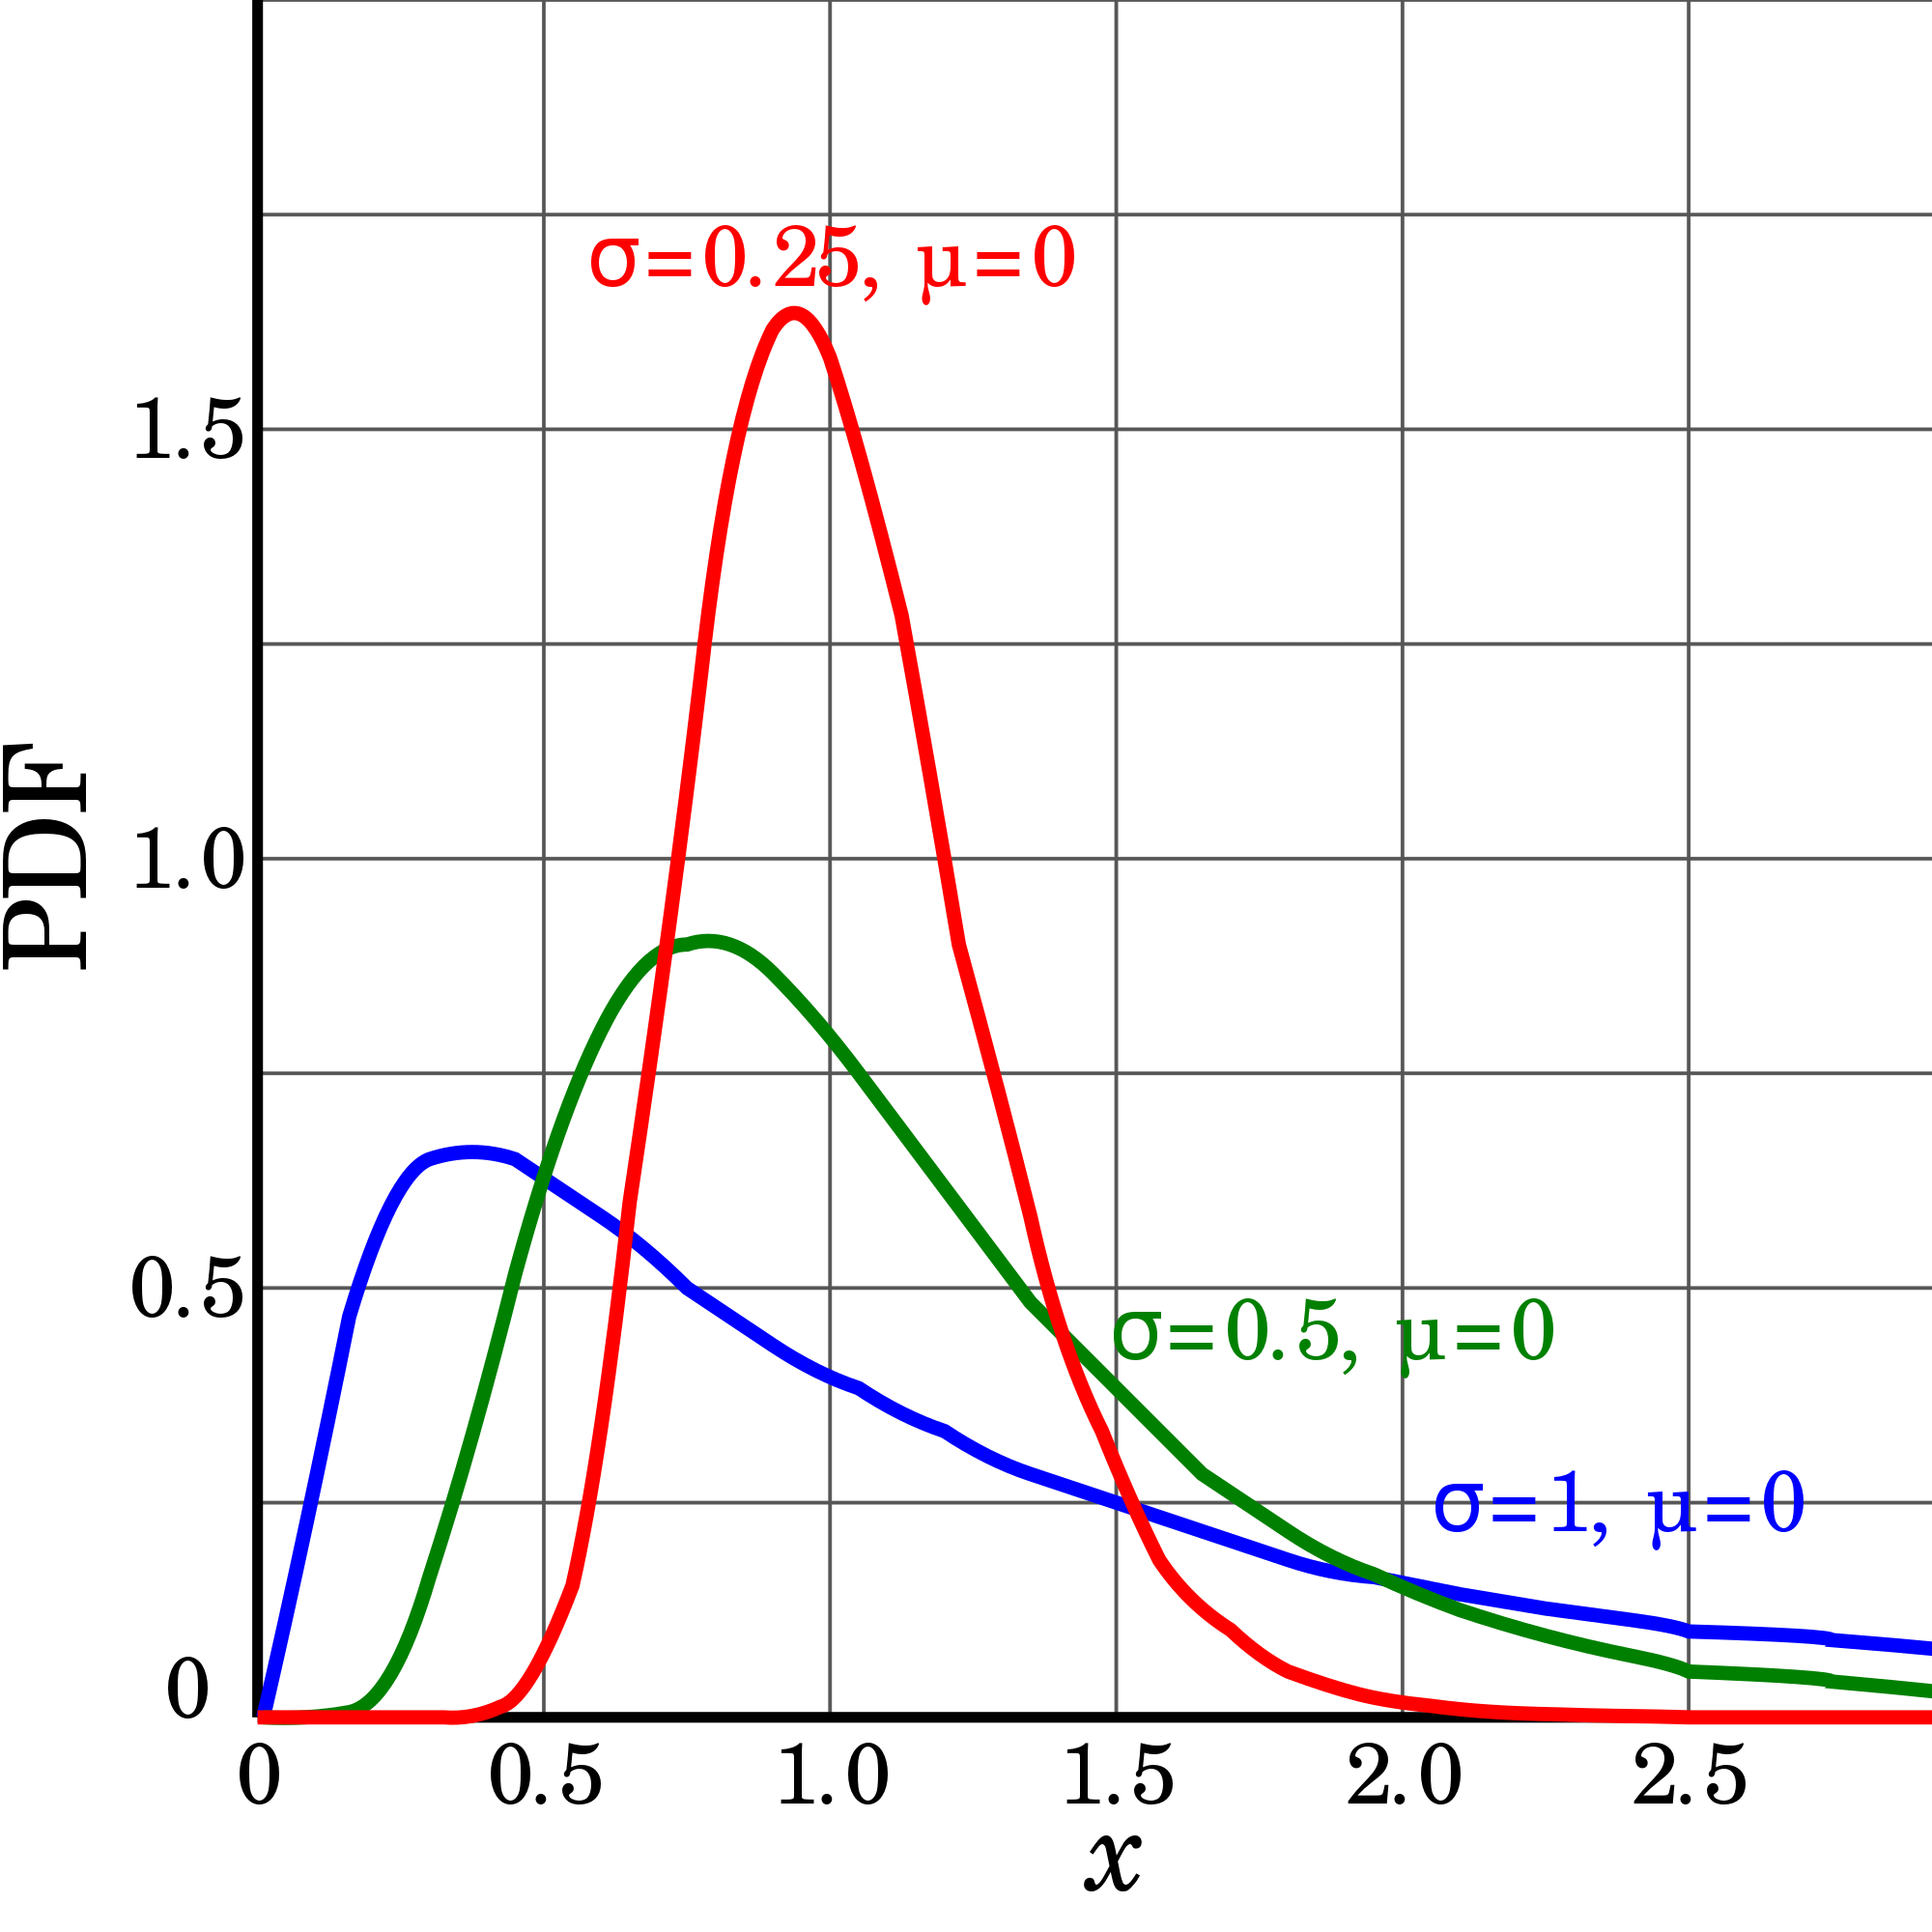
\includegraphics[width=0.65\columnwidth]{{img/2000px-PDF-log_normal_distributions.svg}.png}
\end{frame}

\begin{frame}{Continuous vs discrete actions}
\centering
\begin{tabular}{>{\rowmac}l >{\rowmac}r>{\rowmac}r<{\clearrow}} \toprule
Actions & continuous & discrete \\	\midrule
Sparsity & \textbf{76.3\%} & 73.6\% \\ \midrule
Accuracy & \textbf{99.4\%} & 99.2\% \\
Precision & 98.5\% & \textbf{98.7\%} \\
Recall & \textbf{99.0\%} & 98.3\% \\
F1 & \textbf{99.7\%} & 98.5\% \\
Youden & \textbf{98.5\%} & 97.8\% \\
\bottomrule
\end{tabular}
\end{frame}

\begin{frame}{Comparing with other sampling methods}
Is RL-based sampling better than other simpler techniques?

Comparison against:
\begin{itemize}
\item \textbf{random}: take packets with equal probability
\item \textbf{every \textit{i}th}: take every $i$th packet
\item \textbf{relative first \textit{m}}: for example: take the first 20\% of packets of each flow (not possible if flow length isn't known in advance)
\item \textbf{first \textit{m}}: for example: take the first 10 packets of each flow
\end{itemize}
\end{frame}

\begin{frame}{Comparing with other sampling methods}
\centering
\begin{tabular*}{1.05\columnwidth}{>{\rowmac}l @{\extracolsep{\fill}} >{\rowmac}c>{\rowmac}c>{\rowmac}c>{\rowmac}c>{\rowmac}c<{\clearrow}} \toprule
& RL & random & every $i$th & rel.~first \emph{m} & first \emph{m} \\	\midrule
Sparsity & 76.3\% & 76.3\% & 76.3\% & 76.3\% & 76.3\% \\ \midrule
Accuracy & \textbf{99.4\%} & 96.9\% & 97.8\% & 97.3\% & 98.3\% \\
Precision& \textbf{98.5\%} & 92.4\% & 95.8\% & 93.8\% & 95.6\% \\
Recall & \textbf{99.0\%} & 95.6\% & 95.4\% & 95.5\% & 97.9\% \\
F1 & \textbf{99.7\%} & 94.0\% & 95.6\% & 94.7\% & 96.7\% \\
Youden & \textbf{98.5\%} & 93.0\% & 93.9\% & 93.4\% & 96.4\% \\
\bottomrule
\end{tabular*}
\end{frame}

\begin{frame}{Shared weights}
\begin{itemize}
\item Having \textbf{three neural networks} is a large \textbf{overhead}.
\item During deployment the critic isn't needed so there are two left.
\item What if the classifier, the critic and the actor \textbf{share all weights}?
\end{itemize}
\end{frame}

\begin{frame}{Shared weights}
\centering
\begin{tabular*}{\columnwidth}{>{\rowmac}l @{\extracolsep{\fill}} >{\rowmac}c>{\rowmac}c>{\rowmac}c>{\rowmac}c<{\clearrow}} \toprule
Tradeoff & 0.0 & 0.1 & 0.5 & 1.0 \\	\midrule
Sparsity & 0\% & 77.6\% & 77.6\% & \textbf{78.2\%} \\ \midrule
Accuracy & \textbf{99.5\%} & 99.4\% & 99.3\% & 99.0\% \\
Precision & \textbf{99.4\%} & 99.2\% & 98.6\% & 98.9\% \\
Recall & \textbf{98.5\%} & 98.2\% & 98.7\% & 96.9\% \\
F1 & \textbf{99.0\%} & 98.7\% & 98.6\% & 97.9\% \\
Youden & \textbf{98.4\%} & 97.9\% & 98.2\% & 96.6\% \\
\bottomrule
\end{tabular*}
\end{frame}

\begin{frame}{Visualizing RL's behavior}
Questions:
\begin{itemize}
\item Does the RL pick the \textbf{same packets} for \textbf{each attack} type?
\item Does it pick \textbf{fewer packets} towards the \textbf{end of a flow}?
\item How does the \textbf{confidence increase} during a flow?
\end{itemize}
\end{frame}

\begin{frame}{Benign traffic}
\centering
\includegraphics[width=0.98\columnwidth]{{"img/plot_rl/flows_Jan18_14-06-48_gpu_lstm_module_8.pth_prediction_outcomes_0_3.pickle_10_Normal"}.pdf}
\end{frame}

\begin{frame}{SSH Patator}
\centering
\includegraphics[width=0.98\columnwidth]{{"img/plot_rl/flows_Jan18_14-06-48_gpu_lstm_module_8.pth_prediction_outcomes_0_3.pickle_2_Brute_Force-SSH-Patator"}.pdf}
\end{frame}

\begin{frame}{DDoS Slowloris}
\centering
\includegraphics[width=0.98\columnwidth]{{"img/plot_rl/flows_Jan18_14-06-48_gpu_lstm_module_8.pth_prediction_outcomes_0_3.pickle_7_DoS_-_DDoS-DoS_slowloris"}.pdf}
\end{frame}

\begin{frame}{All samples}
\centering
\includegraphics[width=0.98\columnwidth]{{"img/plot_rl/flows_Jan18_14-06-48_gpu_lstm_module_8.pth_prediction_outcomes_0_3.pickle_15_All_samples"}.pdf}
\end{frame}

\begin{frame}{Steering}
Set a maximum percentage of packets to be sampled (like 50\%) as a \textbf{budget}. Then
\begin{itemize}
\item \textbf{initialize} RL with \textbf{high tradeoff} $\alpha$
\item \textbf{continuously decrease} $\alpha$ towards 0
\item \textbf{stop} if maximum percentage reached
\end{itemize}
\end{frame}

\begin{frame}{Steering}
\centering
  \includegraphics[width=\columnwidth]{{"img/Feb07_17-08-56_gpu_lstm_module_8.pth_global_tradeoff_1.0_steering_step_size_0.1_steering_target_sparsity_0.5_batches_to_consider_for_steering_1000_sampling_rl"}.pdf}
\end{frame}

\section{Discussion}
\begin{frame}{Conclusions}
\begin{itemize}
\item Reinforcement Learning \textbf{works} very well for sampling
\item \textbf{Sharing} all neural network weights makes our approach \textbf{very lightweight}
\item \textbf{Continuous actions} enable skipping \textbf{arbitrarily many} packets and work well
\item \textbf{Steering} allows using a \textbf{fixed cost} budget and then guide the RL to achieve \textbf{maximum accuracy} for that budget
\item \textbf{Other applications} of RL-based packet sampling for traffic classification and other networking tasks?
\end{itemize}
\end{frame}

% -------------
% Last page
% -------------
\makelastslide

\end{document}